% !TEX root = ../00_thesis.tex
%-------------------------------------------------------------------------------
\section{Designing \DRP}
\label{sec:designDetailed}
%-------------------------------------------------------------------------------

We now detail the three building blocks of our solution:
We first describe how \APs and \CPs exchange messages through \bolt~(\cref{subsec:boltAPI}), then we outline the operation of the \blink wireless real-time protocol~(\cref{subsec:details_blink}), and finally we present the detailed design of \DRP~(\cref{subsec:drp}).

%-------------------------------------------------------------------------------
\subsection{Bolt Processor Interconnect}
\label{subsec:boltAPI}

\bolt~\cite{sutton2015Bolt} provides predictable asynchronous message passing between two arbitrary processors, and hence decouples the processors with respect to time, power, and clock domains.
Concrete realizations of Dual-Processor Platforms (\DPP) based on \bolt are depicted in~\cref{append:dpp}.

\cref{fig:bolt_logical} shows a conceptual view of the DPP two message queues with first-in-first-out (FIFO) semantics, one for each direction, form the core of \bolt.
\bolt allows for concurrent \texttt{read} and \texttt{write} operations by \ap and \cp on both queues.

\bolt API includes three functions~(\cref{table:boltAPI}).
The \opwrite function appends a message to the end of the outgoing queue, whereas \opread reads and removes the first message from the incoming queue.
Calling \opflush results in a sequence of \opread operations until the incoming message queue is empty.
The implementation of \opflush is peculiar.
As \bolt allows for concurrent \opread and \opwrite operations, in theory, a \opflush may result in an infinite sequence of {\opread} operations.
To prevent this, the number of {\opread} during a \opflush is upper-bounded by $f_{max}$.
$f_{max}$ is set to the number of messages that fit into one \bolt queue, denoted by $S_{\bolt}$,
\begin{equation}
\label{eq:f_max=M}
f_{max} = S_{\bolt}
\end{equation}
Thus, a \opflush terminates when the incoming queue is found empty or when $f_{max}$ messages have been read out.

By design, \bolt API features predictable execution times, independently of the interconnected processors~\cite{sutton2015Bolt}.
We denote by $C_w$, $C_r$, and $C_f$ the worst-case execution times~(WCETs) of \opwrite, \opread, and \opflush.

\begin{table}
\centering
\caption{\bolt application programming interface (API)}
  {\smaller
  \begin{tabularx}{\linewidth}{@{}c@{\qquad}X@{\qquad}c@{}}
    \toprule
      \textbf{Function} & \multicolumn{1}{c}{\textbf{Description}} & \textbf{WCET} \\
    \midrule
      \texttt{write}
    	& Append a message to outgoing queue
    	& $C_w$ \\[10pt]
      \texttt{read}
      & Read and remove the first message from incoming queue
      & $C_r$ \\[10pt]
      \texttt{flush}
      & Perform up to $f_{max}$ \texttt{read} operations, or until incoming queue is empty
      & $C_f = f_{max}*C_r$\\
    \bottomrule
  \end{tabularx}}
\label{table:boltAPI}
\end{table}

\subsection{Blink Wireless Real-time Protocol}
\label{subsec:details_blink}

\afterpage{
\begin{figure}
 \centering
 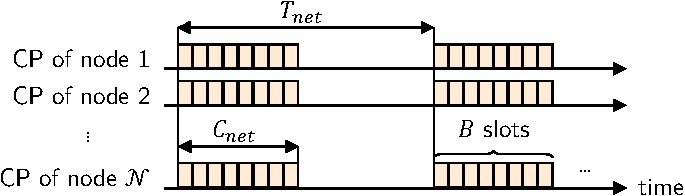
\includegraphics[scale=1]{blink_overview}

 \caption{Operations in \blink are globally time-triggered. \capt{Communication occurs in rounds of equal duration \rlength. Each round consists of a sequence of up to \nslotsmax exclusive time slots, each of which serves to send one message using Glossy floods~\cite{ferrari2011Glossy}.
 The time interval between two consecutive rounds (\rperiod) may vary.
 During a round, the \CP of all nodes in the system participate in the flood.}}

 \label{fig:blink_overview}
\end{figure}
}

In \blink~\cite{zimmerling2017Blink}, wireless multi-hop communication is globally time-triggered and occurs in {rounds} of equal {duration} \rlength~(\cref{fig:blink_overview}).
Each round serves to send up to \nslotsmax messages within exclusive time slots.
In each time slot a message is sent from a given \cp to all other \CPs using Glossy floods, which deliver packets with a probability above 99.9\,\%~\cite{ferrari2011Glossy}.%
%
\footnote{The principle of round-based communication using Glossy floods was introduced in the Low-power Wireless Bus (LWB)~\cite{ferrari2012LWB}. The concept was later adapted in many different flavors~(see the introduction of \cref{ch:baloo}).
\blink is a real-time scheduler for LWB.}
%
The interval between the start of consecutive rounds, denoted by \rperiod, is determined by the host at runtime based on current real-time traffic demands. \rperiodmin and \rperiodmax are implementation-specific bounds on \rperiod.
\blink defines \rperiod and the assignment of messages to rounds such that the number of rounds is minimized and all messages meet their \emph{network deadline} \ndeadlinei between network interfaces (\ie the \CPs).

\blink communication rounds are atomic: during a round, all \CPs are busy executing \blink; other tasks (\eg exchanging messages through \bolt) can only be executed between rounds.
Furthermore, \blink assumes constrained deadlines ($\ndeadlinei \leq \periodi$).
Thus, the network deadline \ndeadlineany must be larger than the minimal round interval and smaller than the flow period \periodany
\begin{equation}
  \rperiodmin \leq \rperiod \leq \ndeadlineany \leq \periodany
\end{equation}

\blink expects periodic message arrivals with a known initial phase for the first packet.
We refer to this as the expected arrival pattern.
For any message matching the expected arrival pattern,
\blink guarantees that, if the message is successfully received at the destination \cp, the message meets its relative network deadline~\ndeadlineany.%

However, we must consider the complete system:
(i)~the message release from the \APs is sporadic with jitter, and
(ii)~\APs and \CPs operate independently~(\feature{Composability}). Thus, there is a mismatch between the periodic arrival pattern assumed by \blink and the actual message arrival at the \CPs.

\subsection{\DRP: Distributed Real-time Protocol}
\label{subsec:drp}

\blink provides real-time guarantees between the network interfaces (\ie the \CPs) assuming periodic message release. \DRP handles the mismatch between the \blink assumptions and the actual message arrival at the \CPs by
(i)~letting the host \emph{assume} that messages are indeed released periodically at the \CPs.
  \blink's communication schedule is computed based on the expected arrival pattern and using an arbitrary initial phase for the flows.
(ii)~analyzing the maximal mismatch between the actual and expected arrival patterns.

This upper-bound represents the maximum extra-delay that a message can suffer before it is scheduled for communication by \blink.
Then, the delay bounds for communication over \bolt and over the wireless network can be combined into a worst-case latency analysis which connects the system parameters (such as the network deadlines and flushing rate of \bolt) with the expected message latency.
\DRP reverts these relations to define values for the system parameters
that guarantee to meet the specified end-to-end deadlines.
\DRP enforces such parameter values using contracts, which are agreed upon at runtime every time a new message flow is registered.

\fakepar{Contracts}
\DRP contracts are key to fulfill the \feature{Timeliness} and \feature{Reliability} requirements. Concretely, these contracts
\begin{itemize}
  \item avoid overflows of message buffers (\eg the \bolt queues) at the source and destination nodes, thus preventing message losses;
  \item ensure that messages are handled ``fast enough'' between the network (\ie \CPs) and the application (\ie \APs) interfaces by the source and destination nodes, such that all messages meet their end-to-end deadlines.
\end{itemize}

To avoid overflows, \DRP defines {maximum time intervals} between two \opflush operations of \bolt by the \CPs and \APs, denoted by $T_f^s$ and $T_f^d$ respectively.
$T_f^s$ is statically set for all \CPs in order not to constrain the achievable end-to-end deadline.
Conversely, $T_f^d$ is adjusted dynamically by the destination nodes upon registration of a new flow.

Providing end-to-end guarantees entails that \DRP decides on the {distribution of responsibilities} among the source node, \blink, and the destination node of a flow \flowi with regard to meeting the end-to-end deadline \deadlinei. To this end, \DRP uses the \emph{deadline ratio}~$r \in (0,1)$, a global parameter chosen at design time.
The joint responsibility of the source and \blink is a function of the source flushing interval $T_f^s$ and the flow's network deadline \ndeadlinei~(computed by \DRP -- \cref{fig:design_overview}). They are responsible for meeting a fraction $r$ of the end-to-end deadline
\begin{equation}\label{eq:function_f}
 f(T_f^s,\ndeadlinei) \; \leq \; r * \deadlinei
\end{equation}
The remaining part of the end-to-end deadline defines the responsibility of the destination, which is a function of its flushing interval $T_f^d$
\begin{equation}\label{eq:function_g}
 g(T_f^d) \; \leq \;  (1-r) * \deadlinei
\end{equation}
In \cref{sec:concrete_realization}, we derive concrete expressions for the functions $f$ and $g$, and we specify how \DRP computes \ndeadlinei and $T_f^d$.
In \cref{sec:drp_evaluation} we illustrate how the choice of the deadline ratio $r$ influences the achievable bandwidth and end-to-end guarantees of our wireless \CPs system.

For each newly admitted flow $\flowi = (\flowsrci,\flowdsti,\periodi,\jitteri,\deadlinei) \in \flowset$, \DRP dynamically establishes two contracts.

\begin{itemize}
	\item \textbf{Source} $\boldsymbol{\leftrightarrow}$ \textbf{Blink}
  \quad
  \flowi's source application, which runs on \apsrc at node  \flowsrci, agrees to write no more messages than specified by the minimum message interval \periodi and the jitter \jitteri. The attached \cpsrc prevents overflows of \bolt and its local message buffer.
	In turn, \blink agrees to serve flow \flowi such that any message matching the expected arrival of \flowi meets its network deadline \ndeadlinei.

	\item \textbf{Blink} $\boldsymbol{\leftrightarrow}$ \textbf{Destination}
  \quad
  \blink agrees to deliver no more messages than specified by \periodi.
	In turn, \cpdst and \apdst agree to read out all delivered messages such that overflows of \bolt and \cpdst's local  buffer are prevented and all messages meet \flowi's end-to-end deadline~\deadlinei.
\end{itemize}

For any flow, if both contracts are fulfilled, all messages that are successfully delivered by \blink will meet their end-to-end deadline. In practice, the contracts fulfillment is guaranteed by a set of \emph{admission tests}, which are performed in sequence upon registration of a new flow, as described next.

\afterpage{
\begin{landscape}
  \begin{figure*}
  \centering
  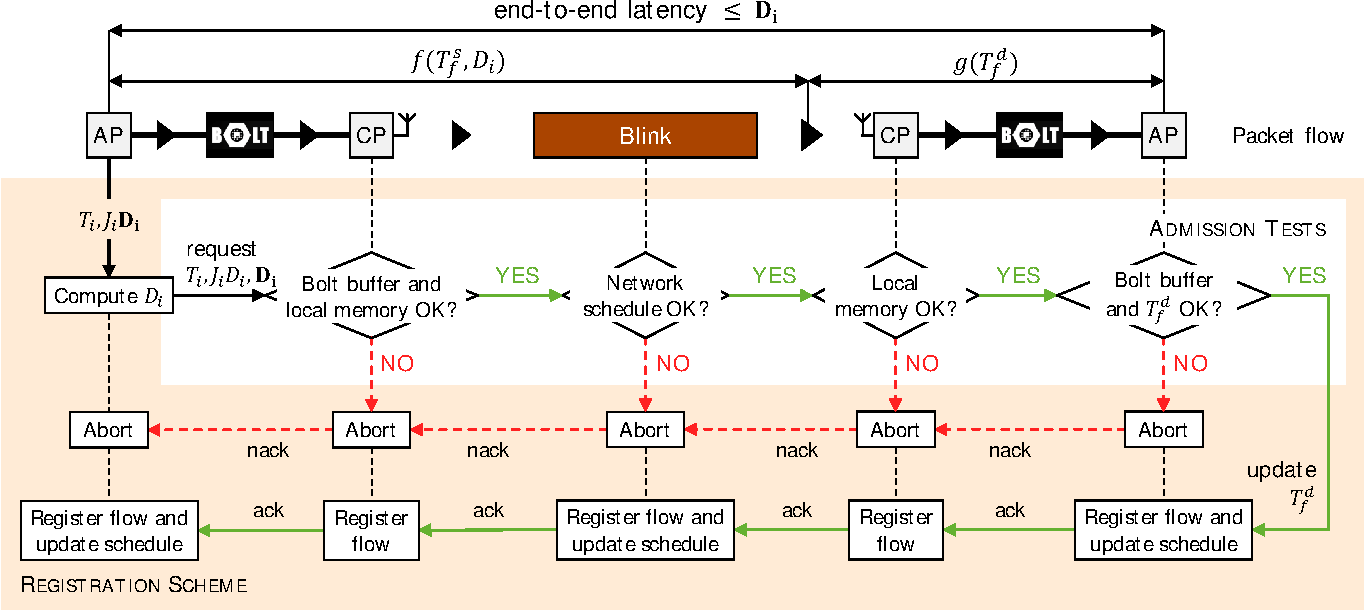
\includegraphics[scale=1]{registration_scheme}

  \caption{Steps and components involved when registering a new flow in \DRP. \capt{Given a request for a new flow $\flowi = (\flowsrci,\flowdsti,\periodi,\jitteri,\deadlinei)$, the source application running on \apsrc at node \flowsrci computes the flow's network deadline \ndeadlinei. Then, all components check one after the other using specific admission tests whether they can admit the new flow. \DRP registers a new flow only if all admission tests succeed, which eventually triggers changes in the runtime operation (the schedule) of \blink as well as of the source and destination application processors \apsrc and \apdst.}}

  \label{fig:design_overview}
  \end{figure*}
\end{landscape}
}

\fakepar{Flow registration}
\cref{fig:design_overview} shows the full procedure for registering a new flow $\flowi = (\flowsrci,\flowdsti,\periodi,\jitteri,\deadlinei)$ in \DRP.
The flow's source application running on \apsrc first computes the network deadline \ndeadlinei (\cref{sec:concrete_realization}) before it writes the request to the attached \cpsrc through \bolt.
\cpsrc uses its admission test to check whether it could still prevent overflows of \bolt and its local memory if \flowi were present.
If so, \cpsrc forwards the request to the host, which checks the schedulability using \blink's admission test~\cite{zimmerling2017Blink}.
If \blink admits the flow, the destination node's \cpdst and \apdst check whether they can prevent overflows of \cpdst's local memory and \bolt, respectively.
Moreover, \apdst re-computes its required flushing interval $T_f^d$ and checks using mainstream schedulability analysis~\cite{buttazzo2011HardRT} whether it can support this new load (in addition to the load incurred by other tasks running on \apdst).
\DRP registers a flow only if all admission tests succeed, which then triggers changes in the runtime operation of \apsrc, \blink, and \apdst.

Flow requests and acknowledgments are sent via dedicated control flows, which are registered by default at bootstrapping for each node in the network.

\afterpage{
\begin{figure}
 \centering
 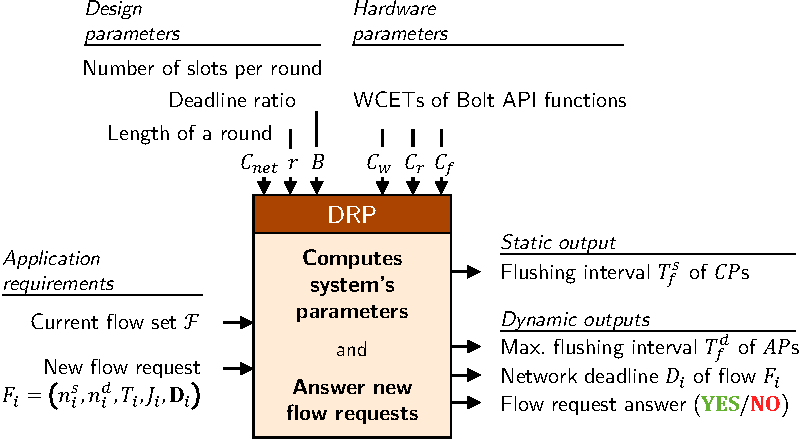
\includegraphics[scale=1]{inputs_outputs}
 \caption{Inputs and outputs of \DRP.
  \capt{Hardware and design parameters are fixed at design time, while the application requirements may change at runtime. \DRP statically computes the flushing interval of \CPs; all other outputs are dynamically computed whenever the flow set $\mathcal{F}$ changes.}}
 \label{fig:procedure_overview}
\end{figure}
}


\fakepar{\DRP procedure}
\cref{fig:procedure_overview} summarizes all the inputs and outputs of \DRP.
Hardware parameters (related to \bolt) and design parameters (\ie the length of a communication round \rlength, the deadline ratio $r$, and the number of slots per round \nslotsmax) are constants known at compile time.
The application's real-time communication requirements may change at runtime as new flows are requested and existing flows are removed. \DRP determines $T_f^s$ statically, while all other outputs are dynamically computed whenever the set of flows changes, according to the procedure illustrated in \cref{fig:design_overview}.
